\chapter{Condition Dependent Performance Based Design and Assessment}

\label{chap-six}

In this chapter, the experimental and analytical program results are used for two application examples. Two examples of the design and assessment of bridges that consider their corrosion is shown.

In addition, the existing methodologies to design structures for life service and assessment for existing structures are evaluated. As will be seen, these methodologies provide tools to consider aging in the structures. However, none of these methodologies directly evaluate corrosion in the structural analysis and design of the structure. Therefore, this study proposes a design and assessment methodology for a single degree of freedom for RC columns subjected to corrosion.

\section{Design of new structures for condition dependent PBD}

One of the biggest challenges in Civil Engineering is to provide infrastructure that is resilient, affordable, and safe. Currently, the design approach assumes that the material properties will remain unchanged throughout the life of the structures. However, built structures age and deteriorate and could potentially lead to the unintended consequence of a structure failing due to aging. Therefore, it is of interest to ensure that new structures are designed to perform to an acceptable level of performance and maintain the level of performance as the structure ages. \fref{fig:ConditionDependent PBD} shows the concept of condition-dependent performance-based design versus the traditional design approach. 

\begin{figure}[htbp]
	\centering
	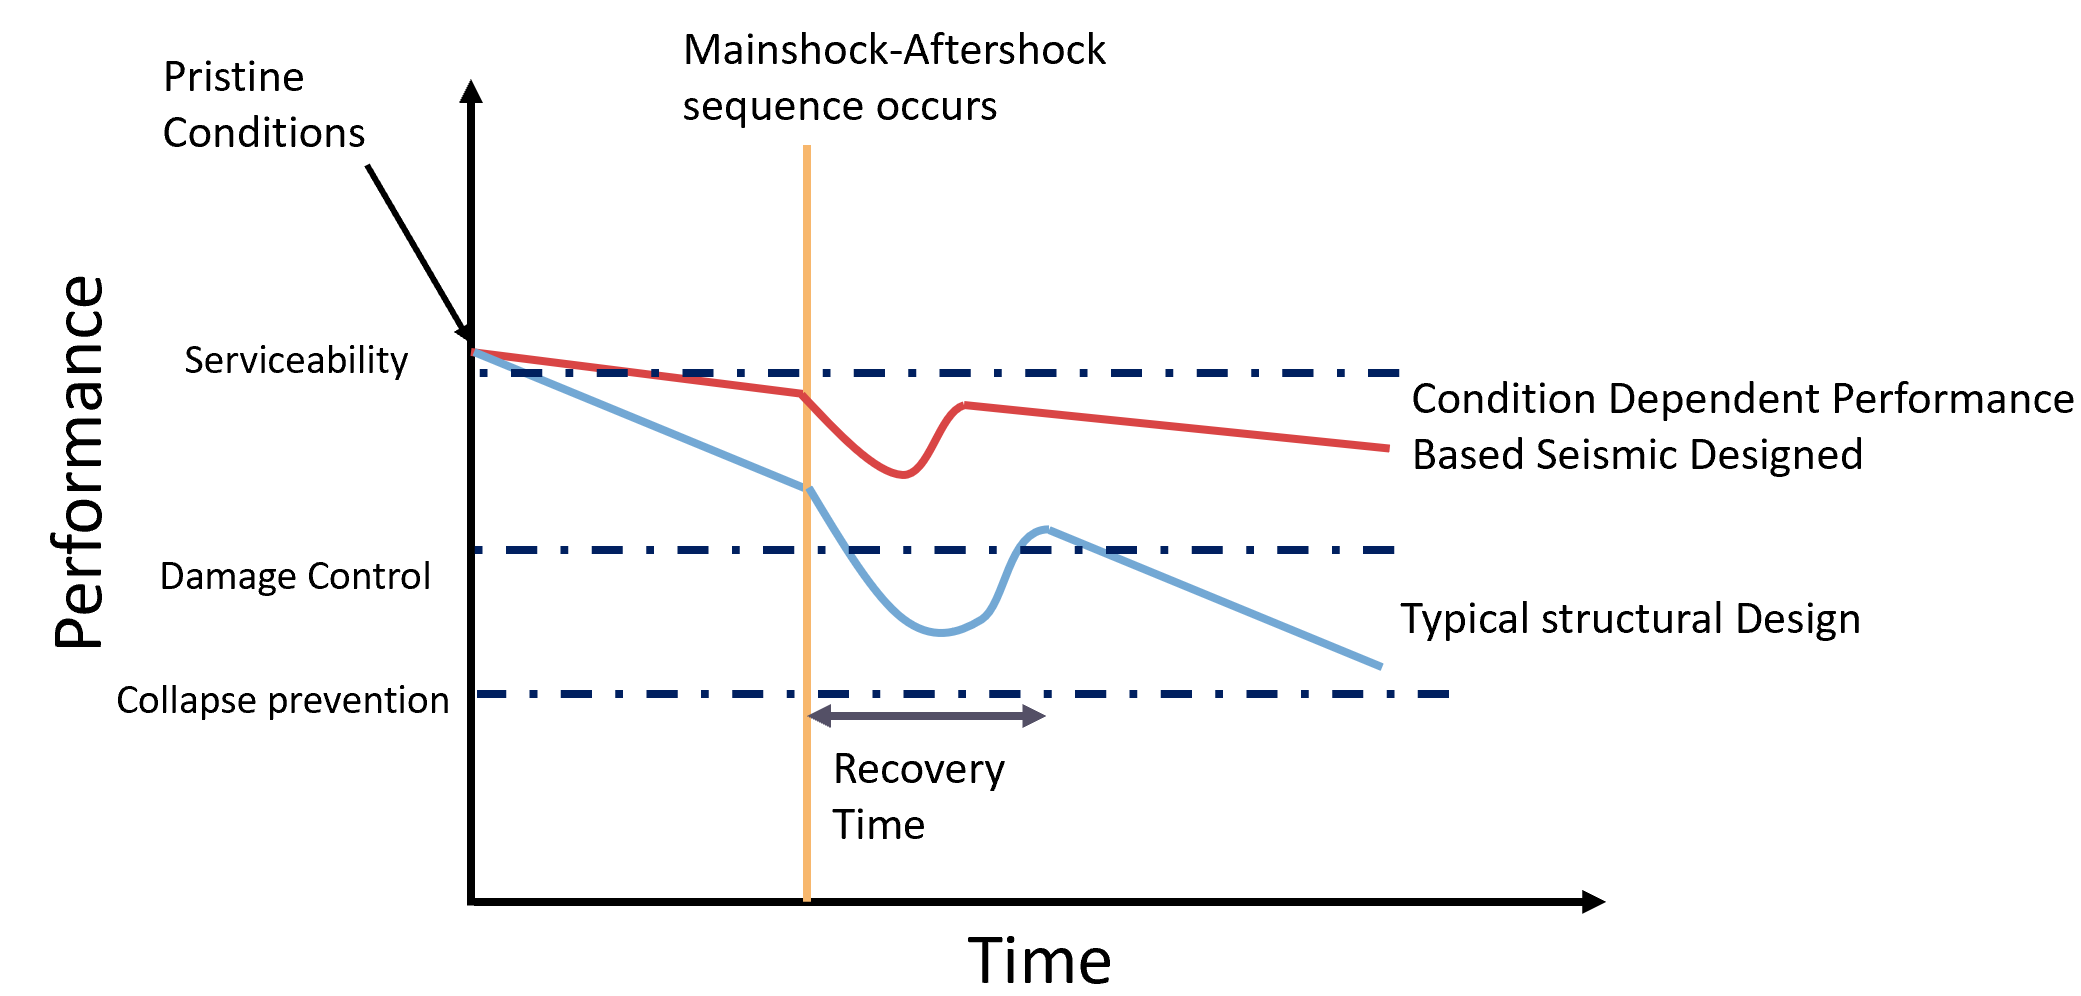
\includegraphics[width=0.9\textwidth]{VAC Thesis 2.0/Chapter-6/figs/CD_DDBD_Concept.png}
	\caption{Philosophy of Condition Dependent Performance Based Design}
	\label{fig:ConditionDependent PBD}
\end{figure}

Currently, existing methodologies provide probabilistic frameworks to design structures for aging. While these methodologies have been used in recent years for significant bridge projects such as the Samuel de Champlain Bridge and the New Bonner Bridge, there is a gap in determining the level of performance as the structure deteriorates.

\subsection{Acceptable level of corrosion for new designs}
The experimental program obtained the equations that relate the degradation of the yield strength and maximum bending strain with corrosion. It was also noticeable in the experimental results that for corrosion levels of 10\% and greater, the bar's strength and capacity to sustain significant buckling levels were significantly reduced. Similarly, the corrosion levels of 10\% and greater in the analytical program significantly increased the likelihood of reaching the damage control and ultimate limit states. Therefore, it becomes evident that for design, a level of corrosion less than 10\% is acceptable for the design of new structures, although a level of corrosion of 5\% or less is desirable.

\subsection{Life Service Design Existing methodologies}

\subsubsection{Life 365}
The Life 365 Consortium III developed the software Life365 to estimate the service life and life-cycle costs of alternative concrete mixture designs and corrosion protection systems\cite{Bentz2003}. The software uses probabilistic analyses of the service life of reinforced concrete structures. The software can calculate the probability distributions within a known time when reinforcement corrosion initiation is expected to occur for a structure. In addition, representative values of the variability of the parameters used in the analysis are provided, such as average temperature throughout the year, Corrosion concentration limits, type of environment (Tidal zone, Spray zone, 800m from the ocean, 1.2 km from the ocean), the type of structure (Parking garage, Urban highway, Rural highway). One of the assumptions is that the deterioration time after corrosion initiation is constant at six years. This program makes it practical to use such distributions in making engineering judgments regarding selecting reinforcement corrosion protection strategies and considering the life costs of different designs. In this study Life 365 is used to accurately determine the time of initiation of corrosion. An example on how the different environments affect the corrosion process is shown in Figure x.x.

\subsubsection{FIB 34 Model Code}
FIB 34 model code addresses Service Life Design (SLD) for plain concrete, reinforced concrete, and pre-stressed concrete structures, focusing on design provisions for managing the adverse effects of degradation. Its objective is to guide bridge stakeholders, practicing engineers, and contractors to ensure the condition of the bridge components and materials is kept above a minimum acceptable level throughout the structure's lifespan. With new bridges having requirements to last for at least 100 years, the design of structures that consider the life service variable has become ever more critical. Therefore, it is crucial to consider one of the primary aging conditions that affect bridges, such as corrosion.

Four different options for SLD are avilable in FIB 34:
\begin{enumerate}
    \item Full probabilistic approach,
    \item Semi probabilistic approach (partial factor design),
    \item Deemed to satisfy rules
    \item Avoidance of deterioration.
\end{enumerate}

An application of the FIB 34 model code has been implemented in a design guide developed by the Federal Highway Administration (FHWA) and the  American Association of State Highway and Transportation Officials (AASHTO) to implement a Service Life Design for Bridges (also referred to as R19A) through the second Strategic Highway Research Program (SHRP2)\cite{SHRP22019}. Multiple tools, products, and training materials aimed at practitioners and state bridge engineers were developed for the implementation effort. In SHRP2-R19A, FIB 34 with a fully probabilistic approach is used to design bridges. The design must ensure that the corrosion is reduced to a 10\% probability of occurrence. In addition, the methodology is implemented to different parts of the structure with exposure zones assigned to them, as shown in Fig X.X. Based on the reliability obtained, changes in the mix design, the reinforcing steel, the cover, and other variables can be made to increase the reliability of the structure. 

This methodology provides a probabilistic methodology to reduce the likelihood of corrosion throughout the structure's life. However, the methodology does not provide a way to directly consider the effect of corrosion on the structure's performance as it ages. Therefore, to ensure that the bridge's condition remains above a minimum acceptable level, it is necessary to evaluate the structure's performance at a given acceptable level of corrosion. The reliability check process is shown in Figure X.X.

\subsection{Direct Displacement Based Design (DDBD) Methodology}
The Direct Displacement Based Design (DDBD) was first proposed by Priestley et al. \cite{Priestley2007}. It is currently one of the design methods accepted in the Proposed AASHTO design Guidelines for Performance-Based Seismic Bridge Design, developed by the National Cooperative Highway Research Program (NCHRP) \cite{NCHRP2020}. DDBD characterizes a structure as an equivalent single degree of freedom system (SDOF) that represents the properties of the structure being designed at peak displacement response. This methodology makes it possible to design a structure to achieve a design limit state under the seismic intensity at the structure's location. This design is later combined with capacity design principles to ensure that the structure behaves as intended by the structural designer. 

The basic steps to apply the DDBD methodology are:
\begin{enumerate}
    \item Determine the structure effective mass ($m_{e}$)
    \item Determine the target displacement. The target displacement can be established by the maximum admissible ductility ($\mu_{adm}$), the maximum drift ($\theta$), or the design limit state (LS).
    \item Calculate the initial design ductility ($\mu_{adm}$)
    \item Calculate the equivalent damping based on the structural element and hysteresis types.
    \item Calculate the effective period of the structure ($T_{eff}$) based on the displacement spectrum at the site of the structure.
    \item Calculate the effective stiffness of the structure as follows:
    \begin{equation}
        K_{eff}=\frac{4\pi^2 m_{e}}{T_{eff}^ 2}
    \end{equation}
    \item Obtain base shear of the structure
\end{enumerate}

The methodology is summarized in \fref{fig:DDBD_CH6}, where the basic steps shown above are explained.
\fref{fig:DDBD_CH6}.
\begin{figure}[htbp]
	\centering
	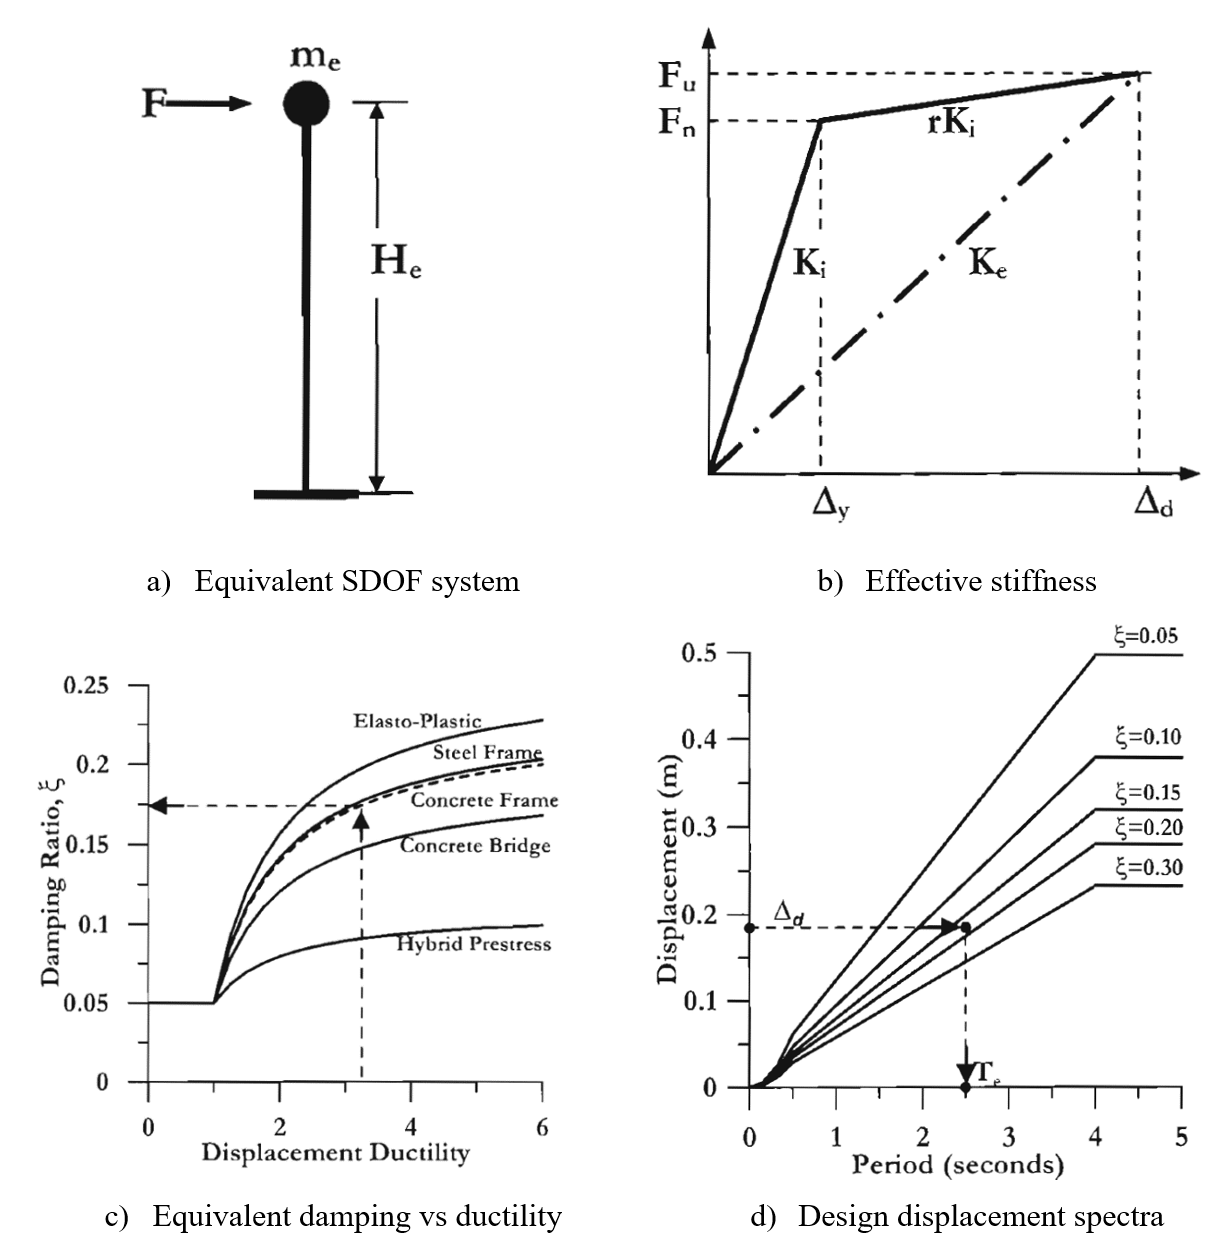
\includegraphics[width=0.75\textwidth]{VAC Thesis 2.0/Chapter-6/figs/DDBD.png}
	\caption{Direct Displacement Based Design (DDBD) methodology}
	\label{fig:DDBD_CH6}
\end{figure}
\subsection{Proposed Condition Dependent DDBD Methodology}

The existing methodologies are robust in predicting the time for initiation of corrosion and obtaining the reliability that the structure will have low probabilities of developing corrosion of the reinforcing steel. However, these tools do not provide a way to estimate the degradation of the structural performance of a structure in the case corrosion occurs. In order to design a structure for corrosion, it is necessary to estimate the highest level of corrosion that will be experienced by the structure. To estimate the highest level of corrosion the main variables are the time of initiation of corrosion and the rate of corrosion. Therefore, a procedure to obtain the level of corrosion and estimate the deterioration of the structure is needed

The proposed methodology consists of:
\begin{enumerate}
    \item Estimate the time of initiation of corrosion. In this study Life 365 is used. An initial concrete mix is made to initiate the design process. Also the water to cement ratio, and cover are specified. The program will calculate the time of initiation of corrosion ($T_{corr}$), based on the design inputs and the type of environment.
    \item The level of corrosion at the end of the life of the structure is determined. First the rate of corrosion needs to be established, as a rule of thumb the rate of corrosion for reinforcing steel is 0.5 mills per year. However, other methodologies can estimate the rate of corrosion based on the water to cement ratio, cover and bar diameter\cite{Weyers1994}\cite{Thoft-Christensen}. The rate of corrosion ($\lambda$) can be expressed as:
    \begin{equation}
        \lambda(t)=0.0005 in/year (t-T_{corr})
    \end{equation}
    Then the reduction of the reinforcing steel can be calculated as:
    \begin{equation}
    d_{b}(t)=d_{bi}-0.0005(t-T_{corr}) (in)
    \end{equation}
    Finally, the level of corrosion, at the end of the life of the structure ($t$), is calculated as:
    \begin{equation}
    CL=1-\left(\frac{d_{b}(t)}{d_{bi}}\right)^2=1-\left(\frac{d_{bi}-0.0005(t-T_{corr})}{d_{bi}}\right)^2
    \end{equation}
    
    \item If $CL$ is less than the admissible level of corrosion $CL_{adm}$, then the concrete mix design, cover or bar diameter can be changed until the corrosion level is acceptable $CL>CL_{adm}$.
    
    \item The effective mechanical properties of the reinforcing steel can be calculated using the expressions developed obtained from the experimental program. The relationships for yield strength and maximum bending strain are replicated here:
    
    \begin{equation}
        f_{y,CL} = f_{y,o}(1-0.0075CL)
        \label{eq.Calderon_Fy_vs_CL_06}
    \end{equation}
    \begin{equation}
        \varepsilon_{b}(CL) = \varepsilon_{o}-0.0045CL
        \label{eq.Calderon_eb_vs_CL_06}
    \end{equation}
    \item The strain limit states for the structure are evaluated with the expressions from \ref{tab:DesignLimitStates}.
    \item Perform the seismic design of the structure using the DDBD methodology.
    \item Final check on the strength of the system $\phi R_{n}>R_{u}$
\end{enumerate}

The design process is outlined in the flowchart shown in\fref{fig:CD-DDBD_CH6}.

\begin{figure}[htbp]
	\centering
	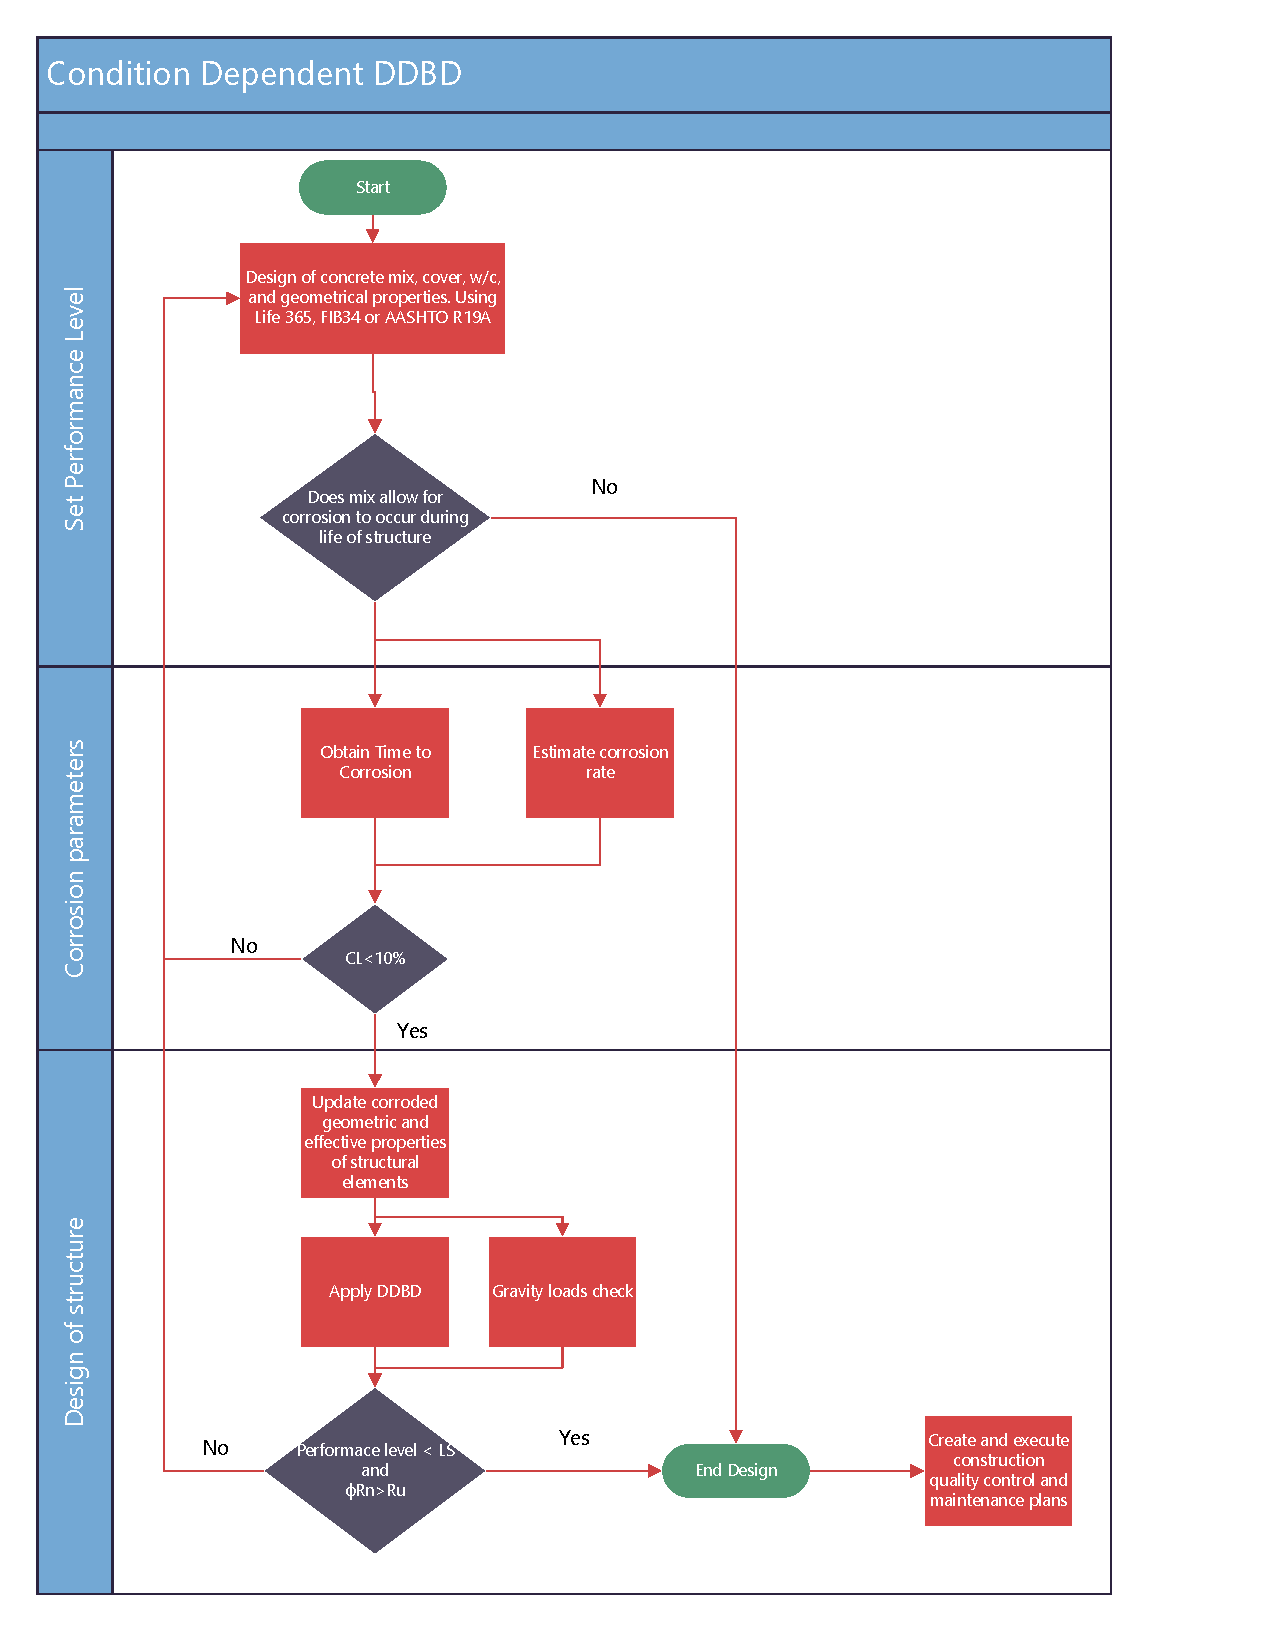
\includegraphics[width=0.875\textwidth]{VAC Thesis 2.0/Chapter-6/figs/CD_DDBD_VictorCalderon.pdf}
	\caption{Proposed Condition Dependent DDBD Methodology flowchart}
	\label{fig:CD-DDBD_CH6}
\end{figure}. 

\subsection{Condition Dependent DDBD application example: SDOF Bridge Pier RC Column}

The example shown below is adapted from Priestley et al \cites{Priestley2007}. The bridge column shown in in Figure X.X. The structure is to be designed for 100 years of life service for the displacement response spectrum shown in Figure X.X. The structure is located within 800 m of the ocean in the city of Anchorage, Alaska.

\textbf{Step 1:} The structure is designed for the environment of 800m from the ocean. The material data used in the structural design are shown in Table X.X. Using life 365 the time of initiation of corrosion is determined to be 18.7 years at the location of the structure. Figure X.X. shows the corrosion degradation that the structure will sustain at 100 years of life service. The resulting level of corrosion is calculated as:
\begin{displaymath}
    CL=1-\left(\frac{d_{bi}-\lambda_{t}(t-T_{corr})}{d_{bi}}\right)^2
\end{displaymath}
\begin{displaymath}
    CL= 1-\left(\frac{1.57 in -0.0005 in/year (100 years -18.7 years)}{1.57}\right)^2=5.03\% \approx 5\%
\end{displaymath}

\textbf{Step 2:} Determine the equivalent mechanical properties of the structure:
\begin{displaymath}
    f_{y,e}=f_{y,o}(1-0.0075\times CL)=420(1-0.0075\times 5.0)=389 MPa
\end{displaymath}
\begin{displaymath}
    \varepsilon_{b}=0.14-0.0045 \times CL = 0.14-0.0045 \times 5.0 = 0.1175 mm/mm
\end{displaymath}

\textbf{Step 3:} Caclulate the damage control and ultimate limit states using equations \ref{eq:es_DamageControl}, and \ref{eq:es_ultimate}.
\begin{displaymath}
    \varepsilon_{s,BB}=0.03+700\rho_{s}  \frac{f_{yhe}}{E_{s}} -0.1\frac{P}{f'_{c}A_{g}}
\end{displaymath}
\begin{displaymath}
    \varepsilon_{s,BB}=0.03+700 (0.00872)  \frac{420 MPa}{200,000 MPa} -0.1\frac{8310 KN}{33MPa (3.1416 m^2)}
\end{displaymath}
\begin{displaymath}
    \varepsilon_{t}=\frac{ln(\frac{\varepsilon_{b}}{0.001})}{\frac{300P}{f'c A_{g}}+\frac{0.7}{\rho_{t}}}=\frac{ln(\frac{0.1175}{0.001})}{\frac{300(8310KN)}{33MPa \cdot 3.1416 m^2}+\frac{0.7}{0.00872}}=0.045
\end{displaymath}

\textbf{Step 4:} Determine the force-displacement response of the structure using cumbia. The displacements for the column at the design limit states are shown below. 


\textbf{Step 5:} Determine the target displacement. The displacements being considered are the damage control limit state, the ultimate limit state and the maximum allowable drift set to $\theta=0.035$.

$Ultimate \to \Delta_{t}=0.54 m \to \mu=4.42$

$Damage Control \to \Delta_{bb} =0.43 m \to \mu=3.5$

$Drift \to \Delta_{\theta}=0.42 m \to \mu=3.42$

$\therefore \Delta_{D}=0.42m$

\textbf{Step 6:} Determine the equivalent damping.
\begin{displaymath}
    \xi_{A}=0.05+0.444\frac{\mu-1}{\mu\pi}=0.05+0.444\frac{3.42-1}{3.42\pi}=0.15
\end{displaymath}

\textbf{Step 7:} Determine the corner period at the effective damping.
\begin{displaymath}
    \Delta_{c,15}=1 m \times \sqrt{\frac{0.07}{0.02+0.15}} = 0.642 m
\end{displaymath}

\textbf{Step 8:} Since $\Delta_{D}<\Delta_{c,15}$, and the corner period $T_{c}=4s$ the effective period can be calculated as shown below.
\begin{displaymath}
    T_{eff}=4s \left(\frac{0.42m}{0.642m}\right)=2.62s
\end{displaymath}

\textbf{Step 9:} Calculate the effective stiffness.
\begin{displaymath}
    K_{e}=\frac{4\pi^2m_{e}}{T_{eff}^2}=\frac{4\pi^2 792.5 KN\cdot s^2/m}{(2.62s)^2}=4557.5 KN/m
\end{displaymath}

\textbf{Step 10:} Calculate the base shear.

$\displaystyle V_{b}=K_{e} \cdot \Delta_{D}= 4557.5 KN/m \times 0.42m = 4557.54 KN$

\textbf{Step 11:} Check strength of the structure.

$M_{u}=V_{b} \times H=4557.54 KN \times 12m = 22,970 KN-m$

From CUMBIA $M_{n} = 26407 KN-m$, using a reduction factor of $\phi=0.9$

$\phi M_{n}>M_{u} \to 23,766.3 KN-m > 22,970 KN-m$

Therefore the structure has sufficient strength to sustain the demands even with a corrosion level of 5\% at 100 years of service life.

\section{Assessment of existing structures considering aging conditions}
For the assessment of structures, it is necessary to have the most accurate information from the structure being assessed. Equally important is that the material behavior is modeled accurately to represent the behavior with corrosion. While current methodologies provide a framework to assess structures in a standardized manner, there is also a gap in how to guide practicing engineers on how to consider aging conditions such as corrosion. Therefore, this section shows the application of a proposed assessment methodology using Direct Displacement Based Assessment for a single degree of freedom RC columns. 

\subsection{Recommendations from the experimental and analytical programs}

The experimental program results showed that corroded reinforcing steel degrades as corrosion increases. Therefore, the methodology proposed here is similar to the design case for structures with corrosion levels less than 10\%. These recommendations are because the loss of strength and performance of corroded reinforcing steel substantially decreased after the value of $CL=10\%$. Therefore, as was shown in the analytical program using a more detailed collection of samples from the existing structure and using a more refined analysis such as Non-Linear Time History analysis (NLTHA) is advised for structures that are found in the field to have corrosion levels higher than 10\%

\subsection{Existing methodologies}

\subsubsection{ASCE 41}

ASCE 41 is the Seismic Evaluation and Retrofit of Existing Buildings code by the American Society of Civil Engineers (ASCE) \cite{ASCE-41-2017}. This code has evolved from FEMA 310 Handbook for the Seismic Evaluation of Building. This code consists of three-tiered procedures for seismic evaluation of existing buildings appropriate for use in areas of any Level of Seismicity. Each tier increases the level of complexity and detail for the structural analysis of the existing structure. The first tier consists of checklists that depend on the type of building and material and the available information to identify deficiencies. If the first tier demonstrates deficiencies, then the second tier is activated. The second tier corresponds to more detailed analysis and verification of the elements that had deficiencies. In the second tier, force-based checks are modified with factors to account for the nonlinearity of the structural elements. During the second tier, if the deficiencies are corroborated, retrofits must be performed, or a more detailed analysis is required to verify the performance of the structures, which triggers the third tier. The third tier corresponds to a more detailed collection of data from the existing structure, and advanced methods of analysis such as Non-Linear Time History Analysis (NLTHA) are required.

While the code provides a framework to evaluate and retrofit existing structures, it is a force-based methodology for tiers 1 and 2, and the code does not guide how to account for aging in the properties of the materials used in the analysis. 

\subsubsection{SLaMA}

Simple Lateral Mechanism Analysis (SLaMA) is a part of the Seismic Assessment of Existing Buildings Guidelines from the New Zealand Society for Earthquake Engineering (NZCEE) \cite{NZSEE2019}. The  Displacement-based assessment (DBA) procedure is used in SLaMA. The procedure focuses on establishing the probable displacement capacity of the primary lateral system. DBA utilizes displacement spectra which can more readily and directly represent the response of a building to earthquake shaking. Displacement-based methods use the same methods as a force-based assessment to determine the force-displacement response of the structure. However, the expected displacement demand is based on the structural characteristics (effective stiffness and equivalent viscous damping) at the assessed displacements rather than on initial elastic characteristics. Displacement spectra set for different levels of elastic damping or ductility are used rather than the acceleration spectra reduced for ductility used for force-based design. The displacement-based approach enables degrading strength and the influence of poor
hysteretic response characteristics to be incorporated in the analysis. Similarly, the concepts can be extended to seismic retrofit design. The basic steps for the SLaMA methodology are enumerated below:

\begin{enumerate}
    \item Assess the structural configuration and load paths to identify critical structural elements, potential structural weaknesses (SWs), and severe structural weaknesses (SSWs).
    \item Calculate the relevant probable strength and deformation capacities for the individual members.
    \item Determine probable inelastic behavior of elements by comparing probable member capacities and evaluating the hierarchy of strength.
    \item Assess the inelastic sub-system mechanisms by extending local to global behavior.
    \item Form a view of the potential governing mechanism for the global building by combining the various individual mechanisms and calculating the probable base shear and global displacement capacity measured at the top of the primary lateral structure. The global displacement capacity will typically be limited to the system with the lowest displacement capacity.
    \item Determine equivalent SDOF system, seismic demand, and \%NBS.
\end{enumerate}

The \%NBS is used as an indicator of risk and defines a structural weakness within the context of SLaMA. For example, SW is an aspect of the building structure and the foundation soils that score less than 100\%NBS. Note that an aspect of the building structure scoring less than 100\%NBS but greater than or equal to 67\%NBS is still considered a structural weakness even though it is considered an acceptable risk. An example of the evaluation of the \%NBS is shown in \fref{}, and the flow chart for the SLaMA procedure is whon in \fref{fig:nbs_CH6}.

This method uses a displacement-based assessment methodology, and therefore a better estimate of the structure's performance is possible. However, similar to ASCE 41, the methodology does not explicitly address how to consider corrosion or aging in assessing the structure.

\begin{figure}[htbp]
	\centering
	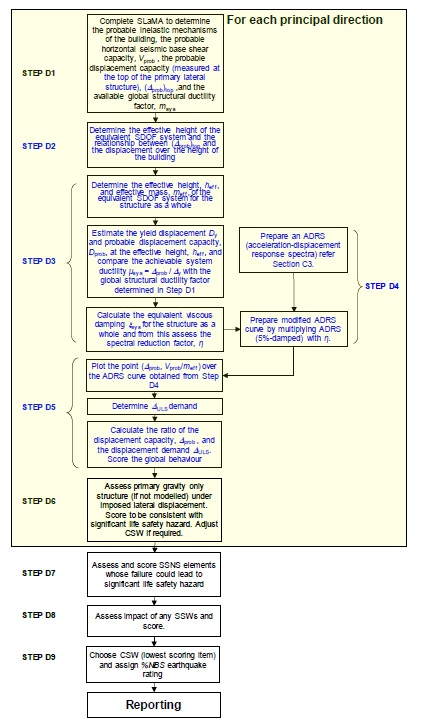
\includegraphics[width=0.75\textwidth]{VAC Thesis 2.0/Chapter-6/figs/SLaMA_methodology.jpg}
	\caption{SLaMA flowchart for the assessment of existing buildings}
	\label{fig:slama_CH6}
\end{figure}
\begin{figure}[htbp]
	\centering
	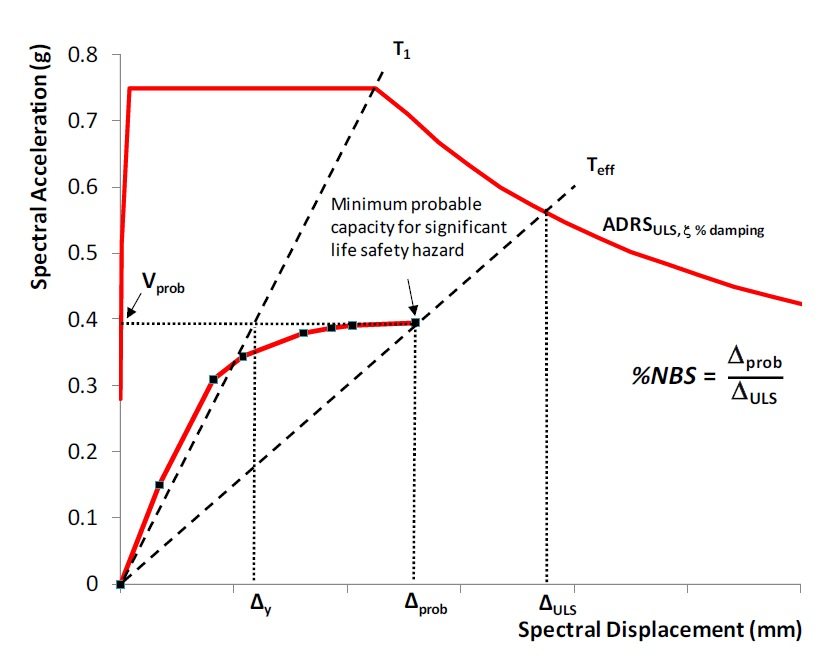
\includegraphics[width=0.60\textwidth]{VAC Thesis 2.0/Chapter-6/figs/nbs_example.jpg}
	\caption{SLaMA \%NBS calculation for assessment}
	\label{fig:nbs_CH6}
\end{figure}
\subsection{Direct Displacement Based Assessment (DDBA) Methodology}

The Direct Displacement Based Assessment (DDBA) uses DDBD principles to assess the compliance of a structure on the premise of the displacement demands and capacities. The advantage of a displacement-based assessment is that the risk of a structure reaching a performance limit state can be readily obtained, incorporating the structure's effective dynamic and structural properties. 

The assesment procedure methodology consistst of:
\begin{enumerate}
    \item Determine the effective mass ($m_{e}$)
    \item Obtain the force-displacement response of the structure using moment-curvature analysis. In this study, CUMBIA is used for this step \cite{Montejo2007}.
    \item From the previously calculated force-displacement response, determine the effective assessment stiffness ($K_{A}=F_{A}/\Delta_{Cap}$) using the displacement ($\Delta_{Cap}$) and force ($F_{A}$) corresponding to the limit state being evaluated.
    \item Determine the effective period as:
    \begin{equation}
        T_{A}=2\pi \sqrt{\frac{m_{e}}{K_{A}}}
    \end{equation}
    \item Determine the displacement ductility ($\mu$)
    \item Determine the effective damping ($\xi_{A}$)
    \begin{equation}
        \xi_{A}=0.05+0.444\frac{\mu-1}{\mu\pi}
    \end{equation}
    \item Calculate the spectral reduction factor $R_{\xi}$ corresponding to $\xi_{A}$, using the expression taken from Priestley at al \cites{Priestley2007}, and shown below:
    \begin{equation}
        R_{\xi}=\left(\frac{0.07}{0.02+\xi_{A}}\right)^{\alpha}
    \end{equation}
    \item Calcualte the equivalent elastic spectral displacement capacity as follows:
    \begin{equation}
        \Delta_{Cap,el}=\frac{\Delta_{Cap}}{R_{\xi}}
    \end{equation}
    \item Calculate the equivalent elastic demand ($\Delta_{dem,el}$) by reading the displacement demand from the spectrum displacement at the effective period of the structure. 
    \item Finally, check the capacity demand displacement ratio, expressed as: 
    \begin{equation}
        C/D= \frac{\Delta_{cap,el}}{\Delta_{dem,el}}
    \end{equation}
    if the ratio is less than one the structure has an satisfactory response, otherwise measures are required to improve the structural performance of the structure.
\end{enumerate}

The DDBA methodology can be summarized in 

\subsection{Proposed Condition Dependent Performance Based Seismic Assessment}

In order to provide tools for practicing engineers to assess aging structures, and specifically include corrosion in their assessment of existing structures, a methodology that uses the Direct Displacement Based Assessment (DDBA) is proposed. Similar to the case of new structures design the degradation of the material properties are included. Some assumptions are necessary to estimate the time of initiation of corrosion of the structures.

The procedure of the Condition Dependent DDBA consists of:

\begin{enumerate}
    \item Obtain information from the existing structure, such as, as built drawings, material certifications, mix design, observations during construction, original structural design calculations.
    \item Historical data, that may include inspection reports, observed deterioration reports.
    \item Site measurements: Corrosion rate (using GalvaPulse), reduced diameter due to corrosion, samples from cocnrete cover to obtain chloride concentration.
    \item Calculate the level ($CL$) of corrosion based on the measured bar diameter ($d_{m}$), and the initial bar diameter ($d_o$) , using the expression: 
    \begin{equation}
        CL=1-\left(\frac{d_{m}}{d_{o}}\right)^2
        \label{eq:CL_diameter}
    \end{equation}
    \item If it is not possible estimate the corrosion level from measured diameter or the rate of corrosion, empirical equations relating the water to cement ratio ($w/c$), bar diameter ($d_{b}$) and cover ($c$) are available in the literature \cite{Weyers1994}\cite{Thoft-Christensen} or by using life 365 \cite{Bentz2003}.
    \item Estimate probable mechanical properties of materials
    \item Apply the Displacement Based Assessment (DBA) procedure
    \item Check the strength of the system with the effective properties of the materials.
\end{enumerate}

\subsection{Condition Dependent DDBA application Example: SDOF Bridge Pier RC Column}

The example shown below is adapted from Priestley et al \cites{Priestley2007}. The bridge column shown in in Figure X.X. presents damage due to corrosion. Th structure was built in the year 2000 the geometry and detailing of the column are shown in Fig X.X. The column is assessed to the ultimate limit state defined in \eqref{eq:es_ultimate} using the DDBA procedure. From a site visit it was determined that the longitudinal reinforcement had reduced to $d_{b,m}=38mm$. The single column pier has a height $H=12m$, and a diameter $D=2m$. The column is assumed to have a rigid foundation and supported on stiff rock. The material properties from the as built drawings are summarized in Table X.X.

\textbf{Step 1:} The corrosion level of the longitudinal reinforcement is estimated:
\begin{displaymath}
    CL=1-\frac{d_{b,m}}{d_{o}}=1-\frac{38}{40}^2=9.75\%
\end{displaymath}

\textbf{Step 2:} The effective mechanical properties of the longitudinal steel are defined
\begin{displaymath}
    f_{y,e}=f_{y,o}(1-0.0075\times CL)=420(1-0.0075\times 9.75)=389 MPa
\end{displaymath}
\begin{displaymath}
    \varepsilon_{b}=0.14-0.0045 \times CL = 0.14-0.0045 \times 9.75 = 0.096 mm/mm
\end{displaymath}

\textbf{Step 3:} Define ultimate limit state
\begin{displaymath}
    \varepsilon_{t}=\frac{ln(\frac{\varepsilon_{b}}{0.001})}{\frac{300P}{f'c A_{g}}+\frac{0.7}{\rho_{t}}}=\frac{ln(\frac{0.096}{0.001})}{\frac{300(8310KN)}{330MPa \times 3.1416 m^2}+\frac{0.7}{0.00872}}=0.04275
\end{displaymath}

\textbf{Step 4:} Obtain the force displacement response for the column using CUMBIA \cite{Montejo2007}. The response is shown in Figure X.X.

\textbf{Step 5:} The effective mass of the structure is calculated
\begin{displaymath}
    m_e=\frac{7500 KN + 810/3}{9.805}=785 KN \cdot s^2/m
\end{displaymath}

\textbf{Step 6:} Calculate the effective assessment stiffness.

\begin{displaymath}
    K_{A}=\frac{F_{A}}{\Delta_{A}}=\frac{2099.4 KN}{0.498 m}=4,215 KN/m
\end{displaymath}

\textbf{Step 7:} Determine the effective period.
\begin{displaymath}
    T_{A}=2\pi \sqrt{\frac{m_e}{K_A}}=2\pi \sqrt{\frac{785}{4215}}=2.724 s
\end{displaymath}

\textbf{Step 8:} Determine the ductility capacity.
\begin{displaymath}
    \mu = \frac{\Delta{A}}{\Delta_{y}} = \frac{0.498}{0.12} = 4.23
\end{displaymath}

\textbf{Step 9:} Determine the effective damping.
\begin{displaymath}
    \xi_{A}=0.05+0.444\frac{\mu-1}{\mu\pi}=0.05+0.444\frac{4.23-1}{4.23\pi}=0.158
\end{displaymath}

\textbf{Step 10:} Calculate the spectral reduction factor.
\begin{displaymath}
     R_{\xi}=\left(\frac{0.07}{0.02+\xi_{A}}\right)^{0.25}=\left(\frac{0.07}{0.02+0.158}\right)^{0.25}=0.792
\end{displaymath}

\textbf{Step 11:} Determine the equivalent elastic spectral displacement.
\begin{displaymath}
     \Delta_{Cap,el}=\frac{\Delta_{Cap}}{R_{\xi}}=\frac{0.498m}{0.792}=0.629
\end{displaymath}

\textbf{Step 12:} Determine the demand spectral displacement, using the displacement spectrum.
\begin{displaymath}
     \Delta_{dem,el}=\frac{\Delta_{c} \times T_{A}}{T_{c}}=\frac{1m \times 2.724s}{1s}=0.681
\end{displaymath}

\textbf{Step 13:} Calculate the capacity demand ratio
\begin{displaymath}
     C/D= \frac{\Delta_{cap,el}}{\Delta_{dem,el}}= \frac{0.629}{0.681}
\end{displaymath}

It can be seen then, that the demand is larger than the capacity and this structure is at high risk of reaching the ultimate limit state. On the other hand. If the calculations are repeated with no corrosion the demand capacity ratio is less than one and appears to be safe. The results highlight the necessity to incorporate the current state of the structure in the assessment of structures. These results are shown graphically in Figure X.X.

\section{Discussion of results}

This chapter showed the versatility of designing and assessing structures using the methodology here proposed. For design, the practicing engineer can readily select the design displacement for the desired level of performance, should the ultimate limit state be too low, the designer can then change the properties of the structure by making the size of the elements larger. 

In the case of assessment it was clear that the methodology shows that the structure with corrosion is at risk of sustaining the ultimate limit state for the assessment displacement spectrum.

\section{Future Work}

While the results shown here are preliminary, they present the possibilities of developing a performance based design methodology that directly accounts for the aging conditions of the structure. More experimental results from physical tests performed on corroded RC columns are needed to determine if there are significant changes on the performance limit states such as serviceability and damage control.